\chapter{System Implementation And Experimental Evaluation}
In order to experimentally evaluate the effectiveness of discussed methods, a set of scenarios were defined and put into experiment. The experiments performed could be classified into two categories:
\begin{itemize}
	\item evaluating the effectiveness of snapshot materialization for computational cost reduction
	\item evaluating the effectiveness of Blockchain for providing trusted data
\end{itemize} 
\section{Data generation and experimental setup}
In order to evaluate our algorithms, we have generated synthetic temporal databases. We have also generated database using the TPCH schema with 1,000,000 tuples in the main table. We also created a set of random database modify, insert and delete updates at 1000 distinct timestamps. This creates a temporal database with 1000 timestamps.
\section{Evaluating snapshot materialization}
\subsection{Linearity of the queries on a temporal table}
Discussed in section \ref{}, preforming queires to create snapshots in a timestamp of interest from the historical data, require visiting all the records before that timestamp and apply all the updates on the table. Over time, when the temporal tables grow in size, performing such computations become expensive and inefficient. To prove it experimentally, we implemented a function to perform such query on our temporal table and record its runtime. Then we performed this query 100 times while sliding the timestamp of the query on the timeline of the temporal table. By sliding the timestamp, in each iteration of the query, more records needed to be visited and more updates needed to be applied. From the runtime records the costline was created which is shown if Figure \ref{fig:linear_time}. 

Figure \ref{fig:linear_time} clearly proves our claim that computation of snapshots on a temporal table requires linear time. The issue of linearity in computation of snapshots makes such tasks on a very large table inefficient. For example in this experiment, the computational cost of 100th query is significantly more expensive than computational cost of 20th query, due to the number of queries which were needed to be visited.

\begin{figure}
	\label{fig:linear_time}
	\centering
	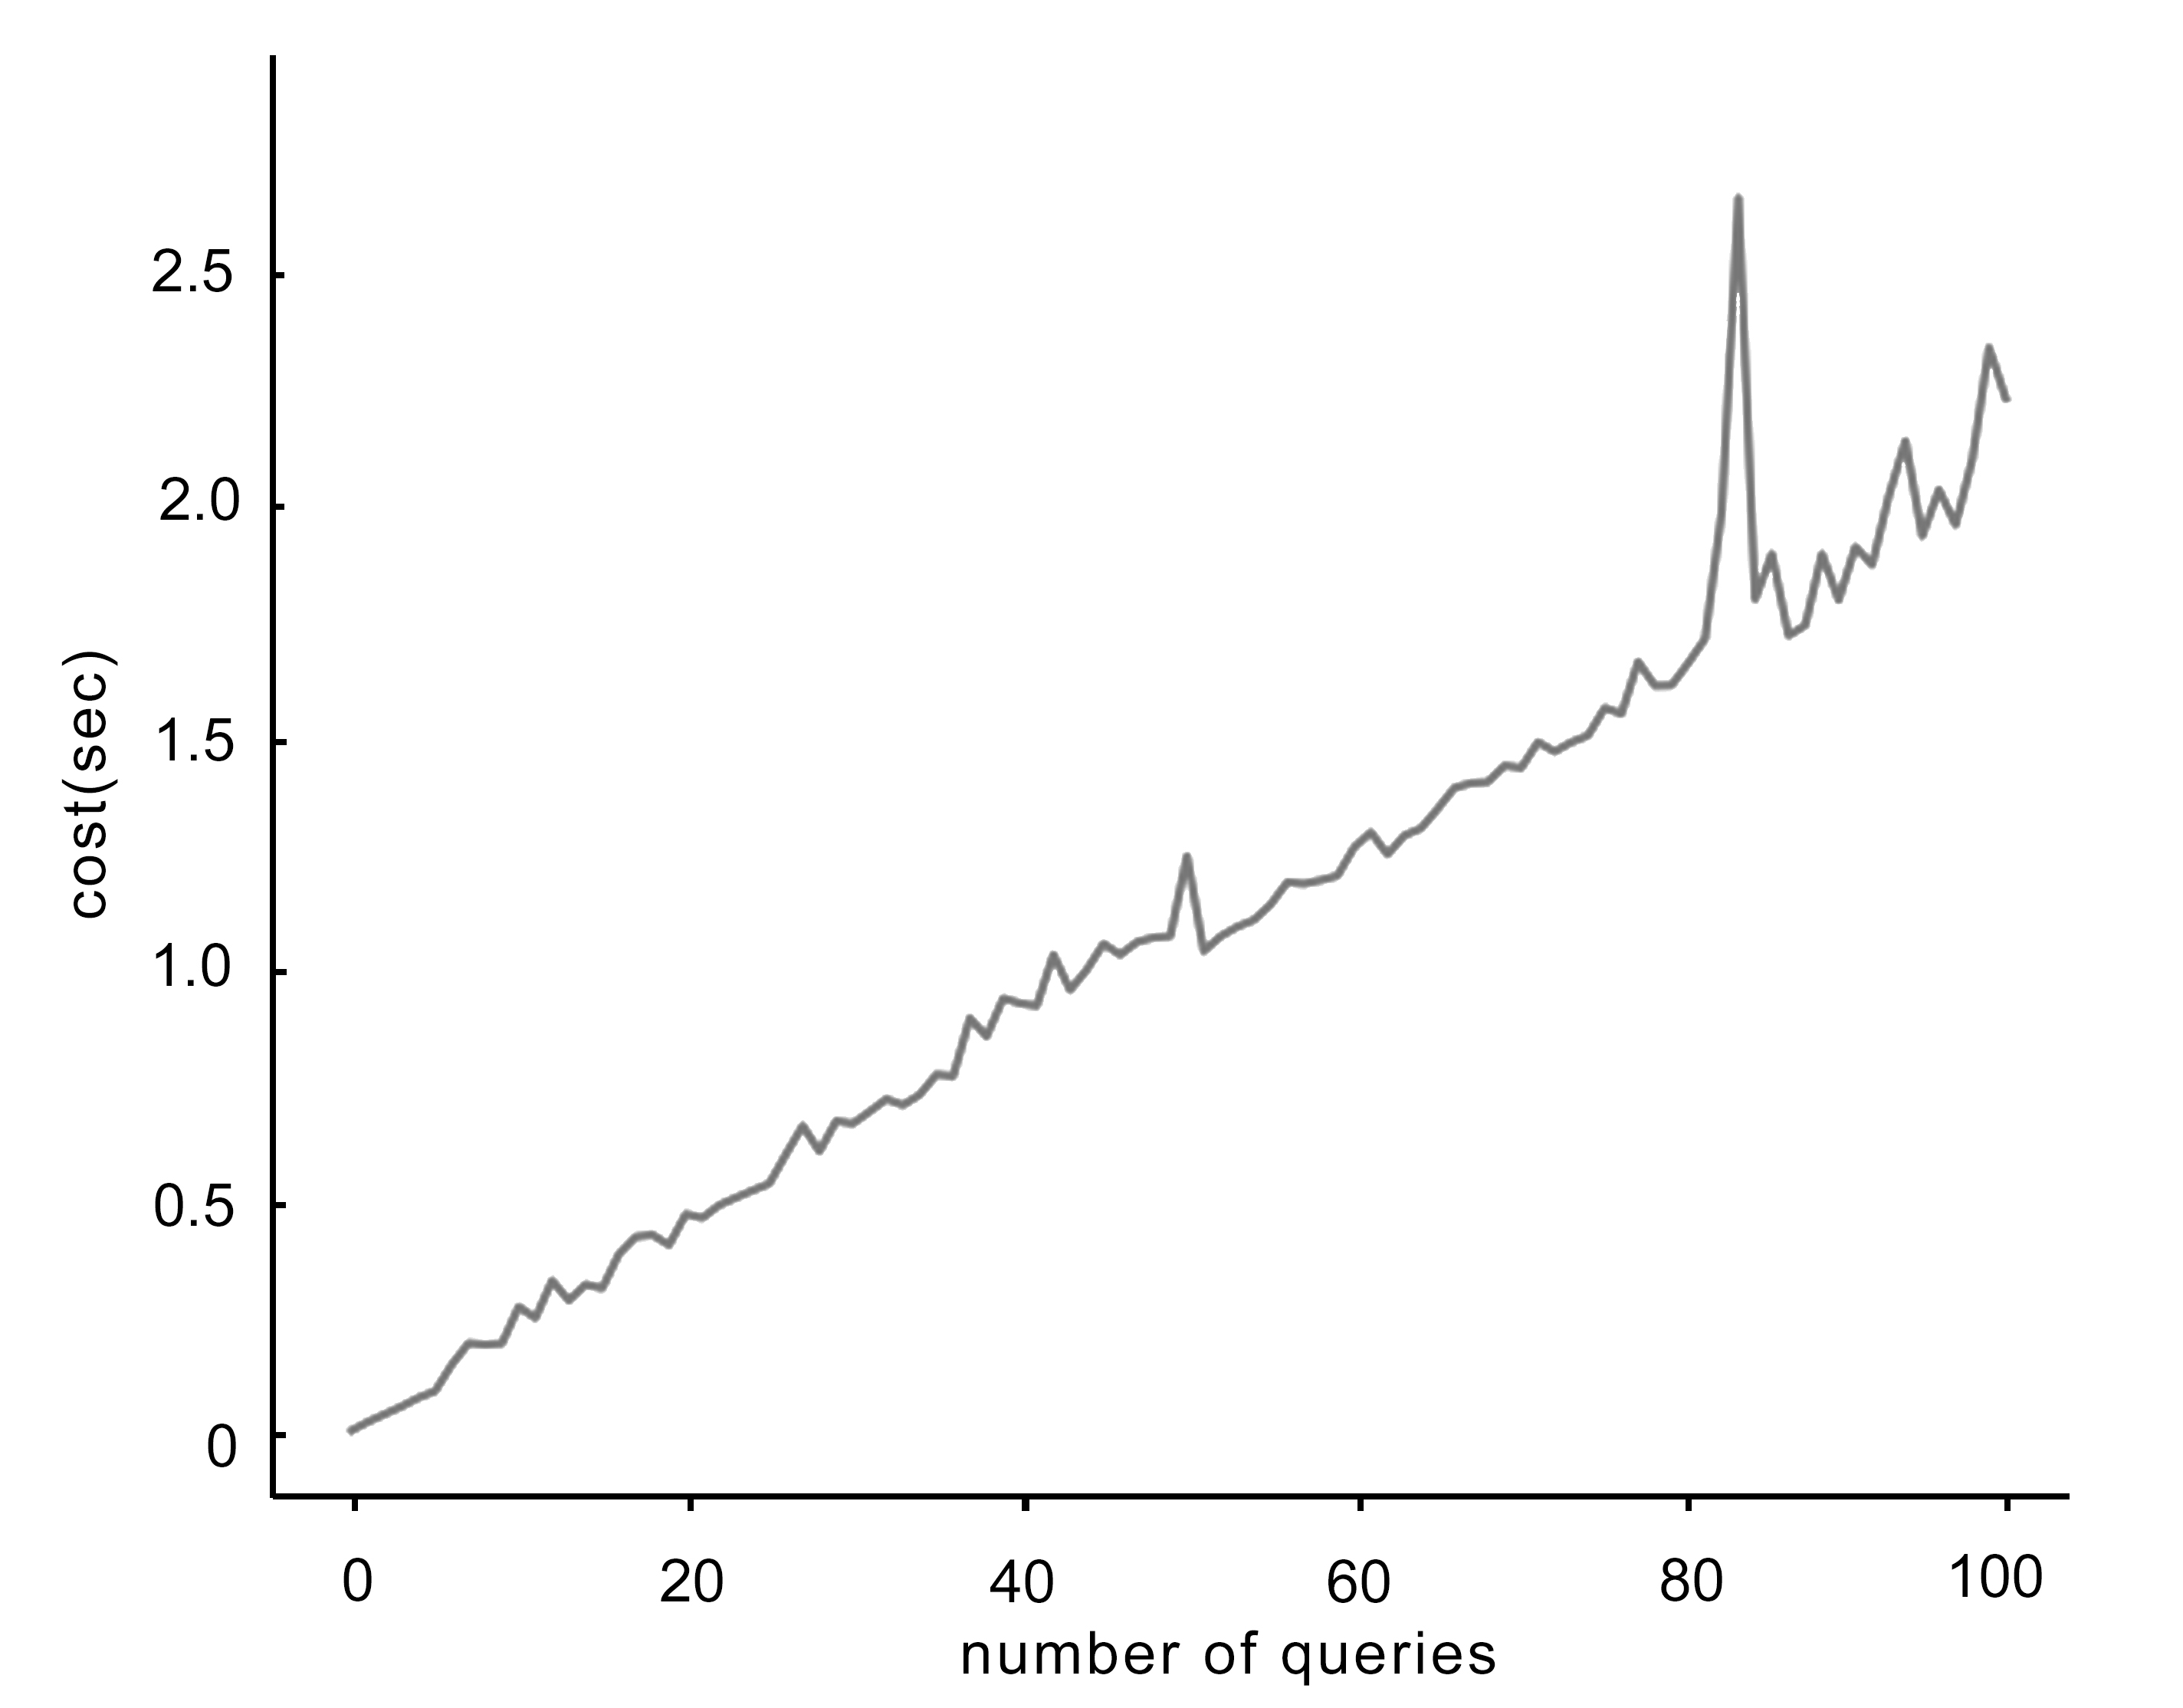
\includegraphics[width=\textwidth]{figs/runtime.jpg}
	\caption{Linear time in computation of snapshots without snapshot materialization}
\end{figure} 

\subsection{Evaluating materialization of a single snapshot}
To illusterate the the optimal position on the timeline to place a single snapshot for materialization, we sampled 60 query timestamps from our temporal database and randomly placed 60 number of queries on its timeline. In the next step we placed a single snapshot that each query materialized to perform the task and recorded the overal cost of queries on that timeline using proposition \ref{}. To see how the position of materialized snapshot may affect the overal cost of query answering, we slided the timestamp of the snashot on the timeline and recorded the overal cost in each snapshot timestamp. The resulted cost line obtained from sliding the snapshot is depicted in Figure \ref{fig:single_snapshot}. 

The resulted cost line shown in Figure \ref{fig:single_snapshot} clearly shows that the position of a snapshot directly affects the overal cost of query answering on the temporal table. In proposition \ref{} we mathematically proved that the median of the queries is the optimal position for snapshot materialization. Therefore in this experiment we calculated the median of the queries which is shown with a red circle in figure \ref{fig:single_snapshot}. As it could be seen, the median of the queries is exactly located in a position where the cost line curve's global minimum is.
\begin{figure}
	\label{fig:single_snapshot}
	\centering
	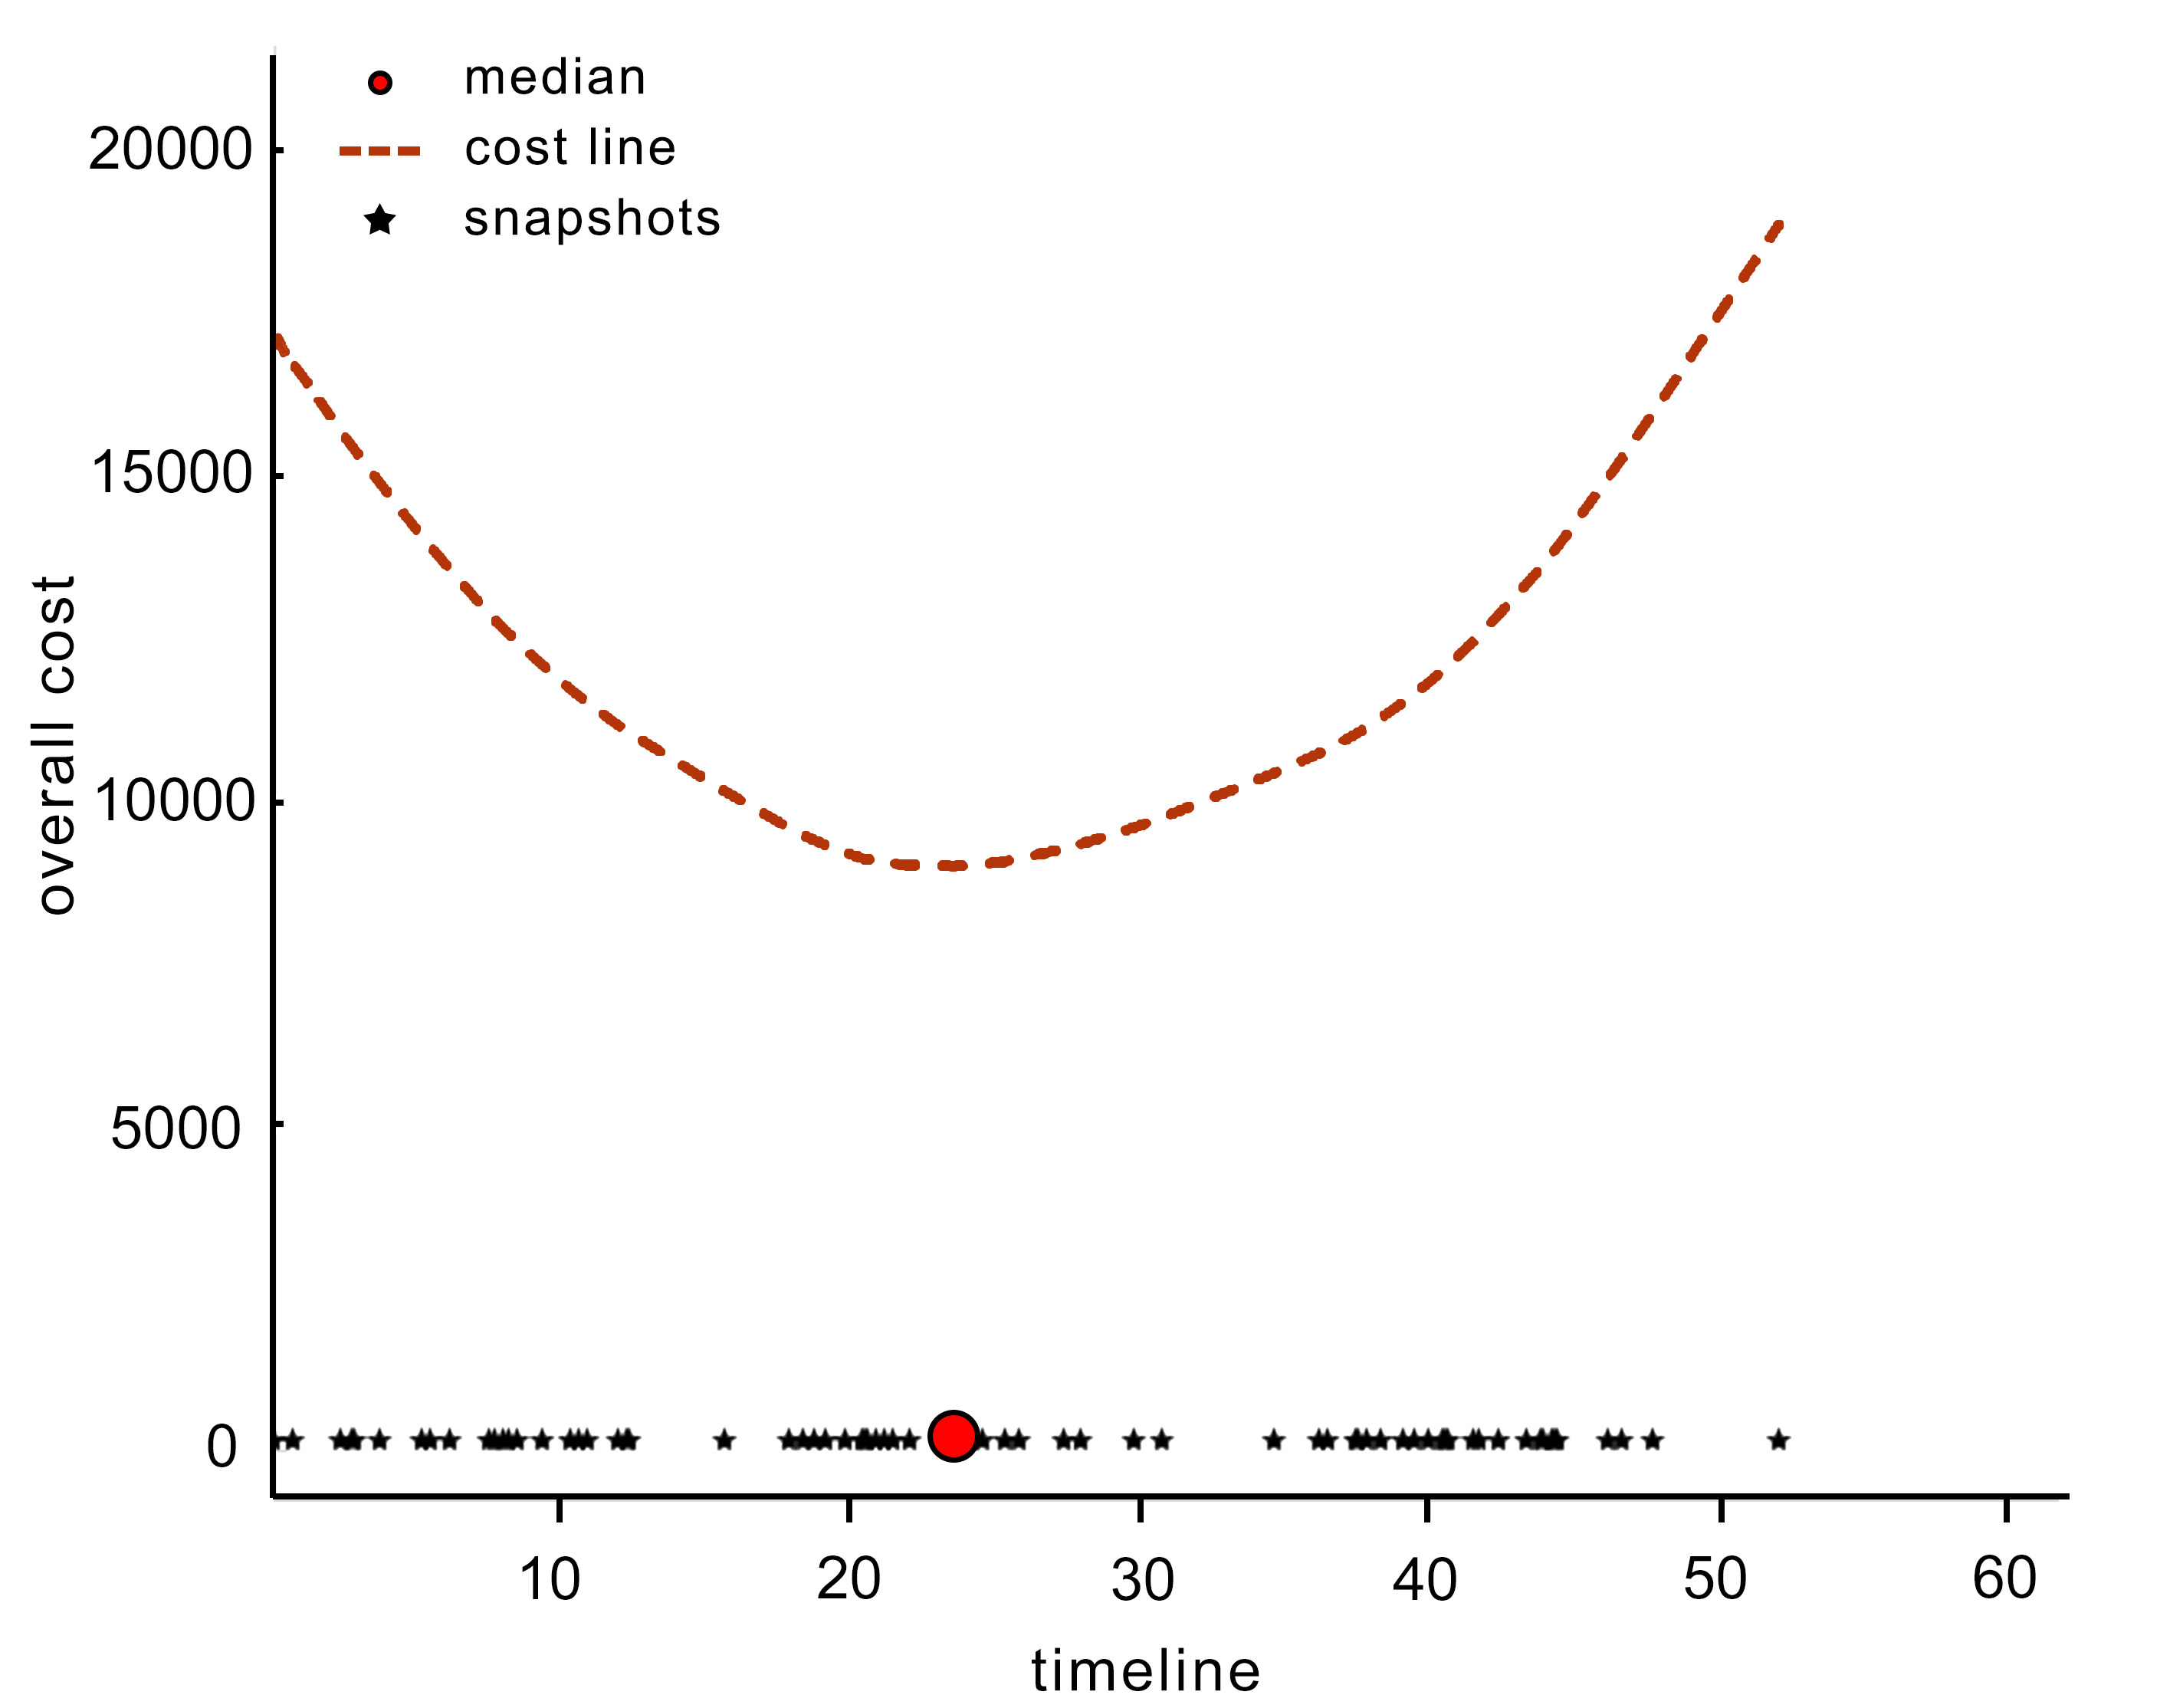
\includegraphics[width=\textwidth]{figs/single_snapshot.jpg}
	\caption{Cost of query answering using a single snapshot over different snaptshot timestamps}
\end{figure} 

\subsection{Evaluating materialization of multiple snapshot}
To evaluate the performance of our optimal snapshot computation, we evaluated the recursive formulation given
by Section \ref{}, the dynamic programming formulation given by Section \ref{} and heuristic method given by Section \ref{}. 

To illustrate that the optimal snapshot placement indeed produces the best query answering performance, we compared the query answering cost of three approaches:
\begin{itemize}
	\item Pick $m$ random timestamps to place the snapshots.
	\item Pick $m$ evenly intervaled timestamps to place the snapshots.
	\item Pick $m$ timestamps computed by dynamic programming.
\end{itemize}

\begin{figure}
	\label{fig:approaches_cost}
	\centering
	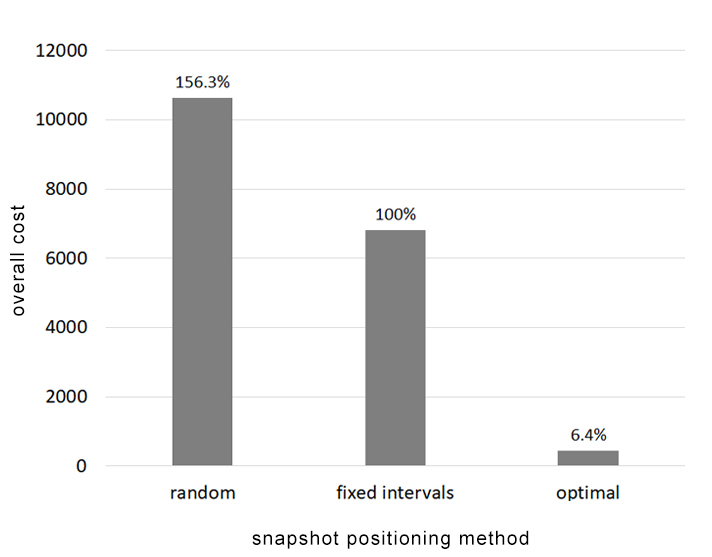
\includegraphics[width=\textwidth]{figs/various_scenarios_cost.jpg}
	\caption{Query answering cost with forty snapshots with various approaches to place snapshots for materialization}
\end{figure} 

Figure \ref{fig:approaches_cost} shows that the placements obtained by dynamic programming clearly beats the other two approaches.

In order to evaluate the effectiveness of $m$ number of snapshots to lower the overal cost of query answering, we recorded the overal cost of queries in various number of snapshots. Figure \ref{fig:snapshots_cost} shows that as the number of snapshots for materialization increases, the overal cost of answering to the queries drops.

\begin{figure}
	\label{fig:snapshots_cost}
	\centering
	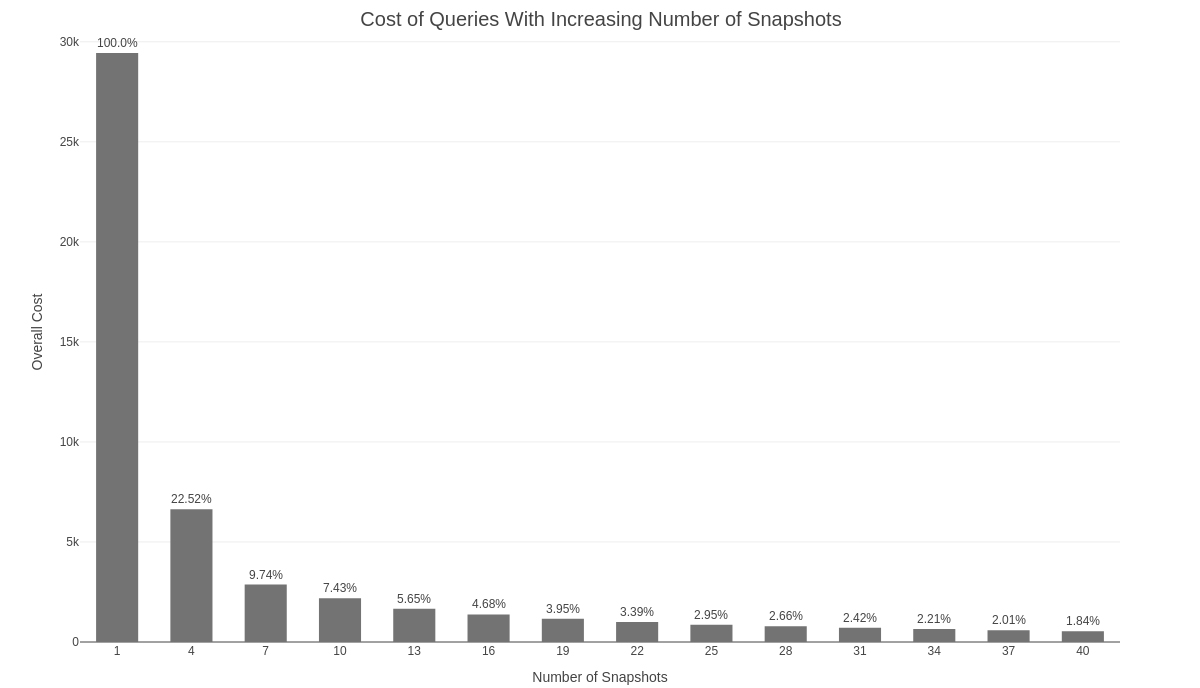
\includegraphics[width=\textwidth]{figs/various_snapshot.jpg}
	\caption{Query answering cost with increasing number of snapshots}
\end{figure} 

\subsection{Evaluating approaches for optimal placement of $m$ snapshots}
As discussed in section \ref{}, we examine 3 approaches to find the optimal timestamps for $m$ number of snashots for materialization. The performed approaches are:
\begin{itemize}
	\item Recursive algorithm.
	\item Dynamic programming.
	\item K-Means clustering.
\end{itemize}


In the first experiment of this category, we evaluate the performance of each approach with respect to variable number of snapshots but fixed number of queries. That is, although the goal of the experiment is to find $m$ number of optimal timestamps for snapshots for materialization, but we start $m=1$ and we increase $m$ in each iteration. For this experiment we sampled 140 number of queries and evalueted the runtime of each approach while increasing the number of requested snapshots.

\begin{figure}
	\label{fig:variable_snapshots}
	\centering
	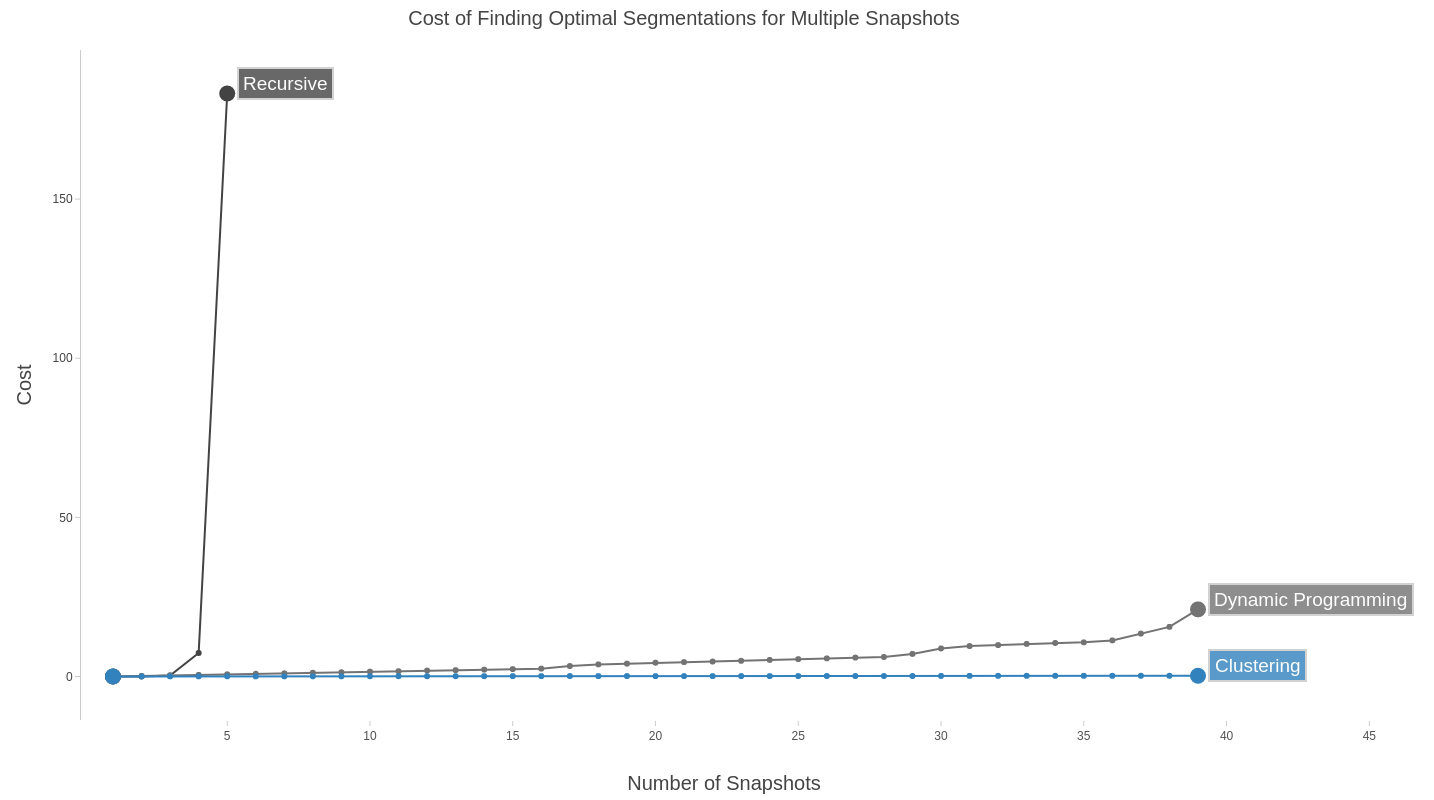
\includegraphics[width=\textwidth]{figs/variable_snapshots.jpg}
	\caption{Optimization time with respect to the number of snapshots}
\end{figure} 


\begin {center}
\begin{table}
	\centering
	\caption{Optimization time with respect to the number of snapshots}
	\label {table:variable_snapshots}
	\begin{tabular}{p{2cm}p{3cm}p{3cm}p{3cm}}
		\hline
		Snapshots & Recursive      & Dynamic  & Clustering \\ \hline
		1 & 0.0002    & 0.01  & 0.01  \\  
		2 & 0.01    & 0.17  & 0.02  \\
		3 & 0.32    & 0.34  & 0.03  \\
		4 & 7.39 & 0.52  & 0.04  \\
		5 & 183.18 & 0.69  & 0.06 \\
		10 & N/A    & 1.52  & 0.08  \\
		15 & N/A & 2.33  & 0.12  \\ 
		20 & N/A & 4.33  & 0.12  \\ 
		25 & N/A & 5.46  & 0.14  \\ 
		30 & N/A & 8.81  & 0.17  \\
		35 & N/A & 10.74  & 0.21  \\
		40 & N/A & 21.09  & 0.24  \\\hline
	\end{tabular}
\end{table}
\end{center}

Figure \ref{fig:variable_snapshots} and Table \ref{table:variable_snapshots} depict the observations of the experiment. The graph shows that in comparison with dynamic programming and K-means clustering, the recursive algorithm is computationally more expensive such that we couldnot utilize this technique to find more than 5 optimal timestamps for snapshots due to the large computational time. 

\begin{figure}
	\label{fig:variable_snapshots_2}
	\centering
	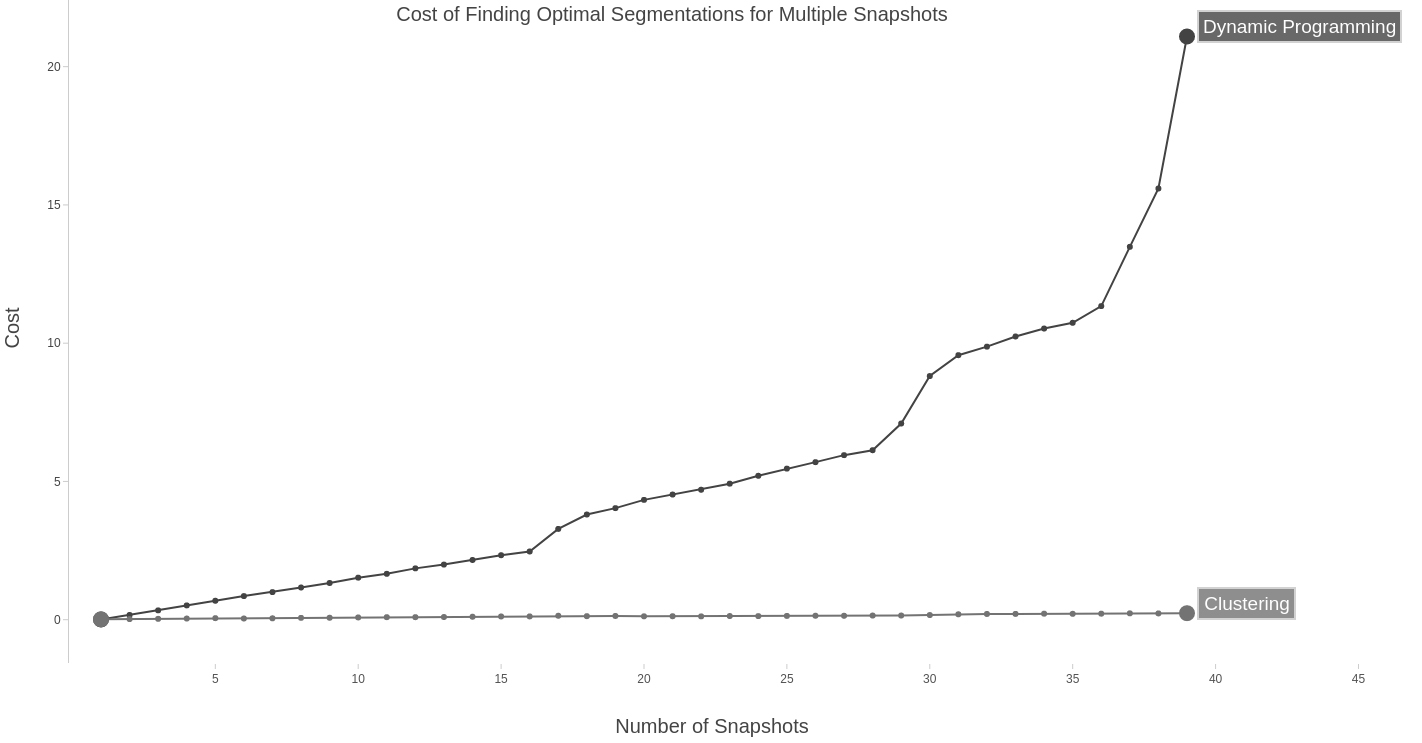
\includegraphics[width=\textwidth]{figs/multiSnapDouble.jpg}
	\caption{Optimization time with respect to the number of snapshots}
\end{figure} 

\begin{center}
\begin{table}
	\centering
	\caption{Optimization time with respect to the number of snapshots}
	\label {table:variable_snapshots_2}
	\begin{tabular}{p{2cm}p{3cm}p{3cm}}
		\hline
		Snapshots  & Dynamic  & Clustering \\ \hline
		1 &   0.01  \\  
		2 &  0.17  & 0.02  \\
		3 &  0.34  & 0.03  \\
		4 & 0.52  & 0.04  \\
		5 &  0.69  & 0.06 \\
		10 &  1.52  & 0.08  \\
		15 & 2.33  & 0.12  \\ 
		20 & 4.33  & 0.12  \\ 
		25 & 5.46  & 0.14  \\ 
		30 & 8.81  & 0.17  \\
		35 & 10.74  & 0.21  \\
		40 & 21.09  & 0.24  \\\hline
	\end{tabular}
\end{table}
\end{center}
Figure \ref{fig:variable_snapshots} and Table \ref{table:variable_snapshots_2}, have a closer look at the dynamic programming and clustering method of finding optimal timestamps. As it could be seen, the clustering method is computationally less expensive than the dynamic programming method.

For the second experiment, we fixed the number of snapshots but made the number of queries variable. Our aim was to observe the performance of each approach as the number of queries grow. For this reason, we calculated 4 number of snapshots for queries ranging from 12 to approximately 180. 

\begin{figure}
	\label{fig:variable_queries}
	\centering
	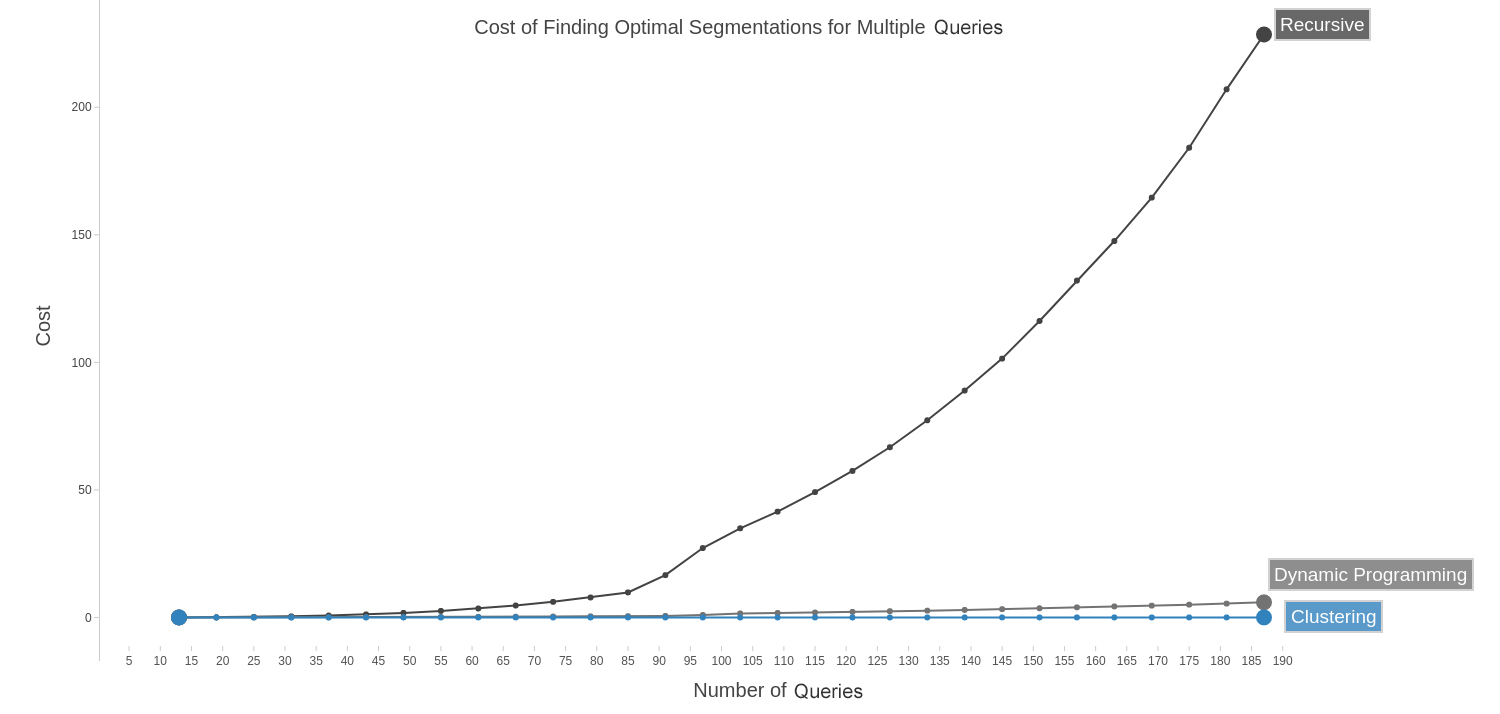
\includegraphics[width=\textwidth]{figs/multi_query.jpg}
	\caption{Optimization time with respect to the number of queries}
\end{figure} 


\begin {center}
\begin{table}
	\centering
	\caption{Optimization time with respect to the number of queries}
	\label {table:variable_queries}
	\begin{tabular}{p{2cm}p{3cm}p{3cm}p{3cm}}
		\hline
		Queries & Recursive      & Dynamic  & Clustering \\ \hline
		13 & 0.05    & 0.01  & 0.02  \\  
		43 & 1.23    & 0.13  & 0.03  \\
		73 & 6.15    & 0.39  & 0.03  \\
		103 & 34.98 & 1.60  & 0.03  \\
		133 & 77.31 & 0.69  & 0.04 \\
		163 & 147.57 & 4.35  & 0.04  \\
		187 & 228.52 & 5.96  & 0.04  \\\hline
	\end{tabular}
\end{table}
\end{center}

Figure \ref{fig:variable_queries_2} and Table \ref{table:variable_queries_2} shows that similar to the previous experiment, recursive algorithm has proven to be expensive in computing the optimal timestamps for the snapshots. To see the difference between the dynamic programming and the clustering method, we compared the performance of both in Figure \ref{} and Table \ref{}. These results also show that utilizing the clustering method is computationally more optimal than the other two method.

\begin{figure}
	\label{fig:variable_queries_2}
	\centering
	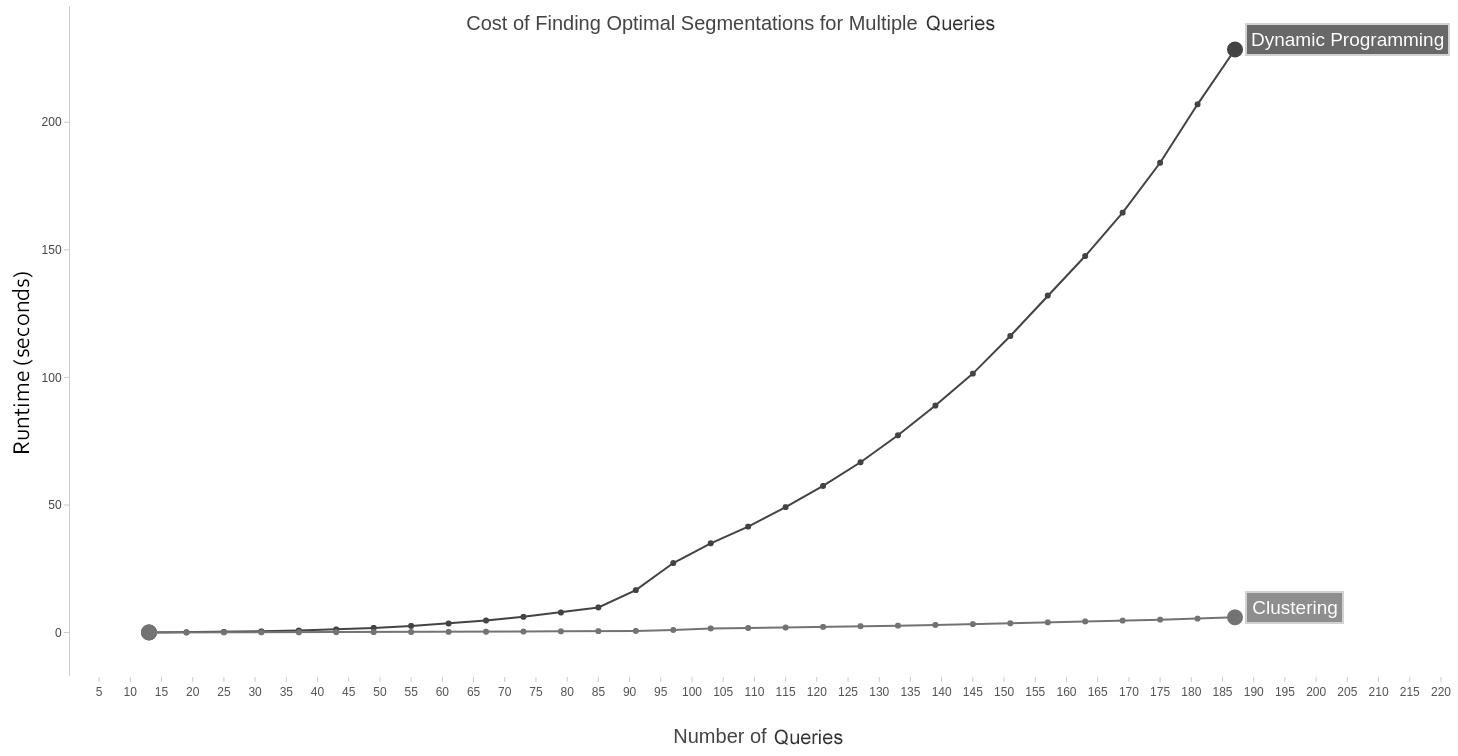
\includegraphics[width=\textwidth]{figs/multi_query_2.jpg}
	\caption{Optimization time with respect to the number of queries}
\end{figure} 


\begin {center}
\begin{table}
	\centering
	\caption{Optimization time with respect to the number of queries}
	\label {table:variable_queries_2}
	\begin{tabular}{p{2cm}p{3cm}p{3cm}p{3cm}}
		\hline
		Queries  & Dynamic  & Clustering \\ \hline
		13 & 0.01  & 0.02  \\  
		43 & 0.13  & 0.03  \\
		73 & 0.39  & 0.03  \\
		103 & 1.60  & 0.03  \\
		133 & 0.69  & 0.04 \\
		163 & 4.35  & 0.04  \\
		187 & 5.96  & 0.04  \\\hline
	\end{tabular}
\end{table}
\end{center}

\subsection{Evaluating the heuristic method}
In the previous section we showed that the heuristic method (K-Means clustering method in this case) is computationally more favorable than the recursive algorithm and dynamic programming method. However unlike recursive algorithm and dynamic programming which compute the exact optimal timestamps for the snapshots, the heuristic method approximates the optimal timestamps. Because of this, in the heuristic method, finding the most optimal timestamps for the snapshots is not guaranteed. Therefore a comparison was needed to evaluate if the heuristic method could be chosen over the other two method.

We previousely showed that as the number of snapshots grow, the overall cost of answering to the queries drops. In this experiment, we compared the outcome of the dynamic programming and K-Means clustering method in varying number of snapshots and see how increasing the number of snapshots affect the overall cost of query answering in both methods. As it could be seen in Figure \ref{fig:dynamic_vs_heuristic} and Table \ref{}, the outcome of dynamic programming and heuristic method is slightly different but the result is satisfactory.

\begin{figure}
	\label{fig:dynamic_vs_heuristic}
	\centering
	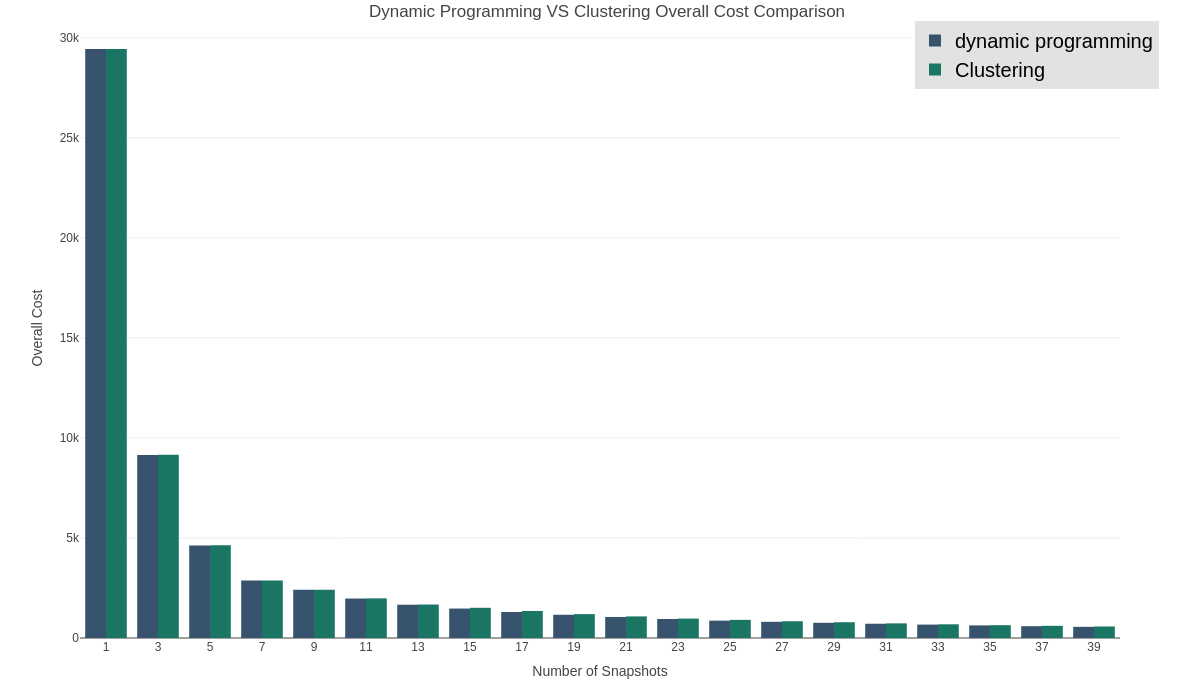
\includegraphics[width=\textwidth]{figs/dynamic_vs_clustering.jpg}
	\caption{Comparing the outcome of dynamic programming with the heuristic method}
\end{figure} 

\section{Observations and conclusion}